\begin{frame}[fragile]\frametitle{Review: Three Methods}
  \begin{itemize}
    \item \textbf{Algebraic}: elimination, substitution
    \item Solve $2x + 3y = 6$, $x - y = 3$ by manipulation
    \item \textbf{Graphical}: plot lines, find intersections
    \item Three cases: unique, no solution, infinite solutions
    \item \textbf{Transformation}: $T(x,y) = (x+2y, 3x-y)$
    \item Geometric interpretation: square to parallelogram
    \item \textbf{Matrix notation}: $\begin{pmatrix} a & b \\ c & d \end{pmatrix} \begin{pmatrix} x \\ y \end{pmatrix}$
  \end{itemize}
\end{frame}

\begin{frame}[fragile]\frametitle{Composition of Transformations}
  \begin{itemize}
    \item Two transformations: $T: xy \to XY$ and $U: XY \to X'Y'$
    \item Composition: $U \circ T: xy \to X'Y'$
    \item Matrix form: $(U \cdot T) \mathbf{x}$
    \item \textbf{Critical}: Matrix multiplication is NOT commutative
    \item $TU \neq UT$ in general
    \item Order matters when composing transformations
    \item Example: rotation then reflection $\neq$ reflection then rotation
  \end{itemize}
\end{frame}

\begin{frame}[fragile]\frametitle{Transformation Examples}
  \begin{columns}
    \begin{column}[T]{0.6\linewidth}
      \begin{itemize}
        \item \textbf{180° rotation}: $T(x,y) = (x, -y)$
        \item Matrix: $\begin{pmatrix} 1 & 0 \\ 0 & -1 \end{pmatrix}$
        \item Flips across x-axis
        \item \textbf{90° rotation}: $U(x,y) = (y, x)$
        \item Matrix: $\begin{pmatrix} 0 & 1 \\ 1 & 0 \end{pmatrix}$
        \item Swaps x and y coordinates
      \end{itemize}
    \end{column}
    \begin{column}[T]{0.4\linewidth}
      \begin{center}
        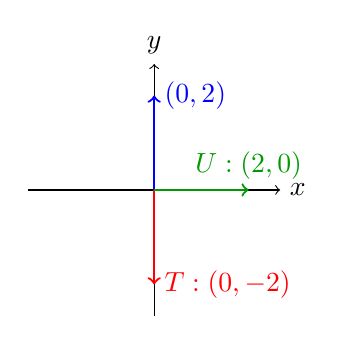
\begin{tikzpicture}[scale=0.8]
          \draw[->] (-2,0) -- (2,0) node[right] {$x$};
          \draw[->] (0,-2) -- (0,2) node[above] {$y$};
          \draw[->,blue,thick] (0,0) -- (0,1.5) node[right] {$(0,2)$};
          \draw[->,red,thick] (0,0) -- (0,-1.5) node[right] {$T: (0,-2)$};
          \draw[->,green!60!black,thick] (0,0) -- (1.5,0) node[above] {$U: (2,0)$};
        \end{tikzpicture}
      \end{center}
    \end{column}
  \end{columns}
\end{frame}

\begin{frame}[fragile]\frametitle{Matrix Multiplication Rule}
  \begin{itemize}
    \item Row-column multiplication
    \item $\begin{pmatrix} a & b \\ c & d \end{pmatrix} \begin{pmatrix} e & f \\ g & h \end{pmatrix} = \begin{pmatrix} ae+bg & af+bh \\ ce+dg & cf+dh \end{pmatrix}$
    \item First row times first column: $ae + bg$
    \item Example: $TU = \begin{pmatrix} 1 & 0 \\ 0 & -1 \end{pmatrix} \begin{pmatrix} 0 & 1 \\ 1 & 0 \end{pmatrix} = \begin{pmatrix} 0 & 1 \\ -1 & 0 \end{pmatrix}$
    \item Represents combined transformation
    \item Compute $UT$ yourself: different result
  \end{itemize}
\end{frame}

\begin{frame}[fragile]\frametitle{Coordinate Systems}
  \begin{itemize}
    \item \textbf{Cartesian coordinates}: $(x, y)$
    \item Specify horizontal and vertical distances
    \item Good for rectangular geometries
    \item \textbf{Polar coordinates}: $(r, \theta)$
    \item Specify distance and angle from origin
    \item Good for circular symmetries
    \item Also: spherical (3D spheres), cylindrical (3D cylinders)
    \item Different problems need different coordinates
  \end{itemize}
\end{frame}

\begin{frame}[fragile]\frametitle{Polar to Cartesian Conversion}
  \begin{columns}
    \begin{column}[T]{0.6\linewidth}
      \begin{itemize}
        \item Given: distance $r$ and angle $\theta$
        \item Cartesian coordinates: $x = r \cos \theta$
        \item $y = r \sin \theta$
        \item Example: $r=5$, $\theta=30°$
        \item $x = 5 \cos 30° \approx 4.33$
        \item $y = 5 \sin 30° = 2.5$
        \item Point $(4.33, 2.5)$ in Cartesian
      \end{itemize}
    \end{column}
    \begin{column}[T]{0.4\linewidth}
      \begin{center}
        \begin{tikzpicture}[scale=0.9]
          \draw[->] (0,0) -- (4,0) node[right] {$x$};
          \draw[->] (0,0) -- (0,3) node[above] {$y$};
          \draw[->,thick,blue] (0,0) -- (3,1.7) node[midway,above left] {$r$};
          \draw[dashed] (3,1.7) -- (3,0) node[midway,right] {$y$};
          \draw[dashed] (3,1.7) -- (0,1.7);
          \draw (0.8,0) arc (0:30:0.8) node[midway,right] {$\theta$};
          \node at (1.5,-0.3) {$x$};
        \end{tikzpicture}
      \end{center}
    \end{column}
  \end{columns}
\end{frame}

\begin{frame}[fragile]\frametitle{Why Abstract Mathematics?}
  \begin{itemize}
    \item Coordinate systems depend on geometry
    \item Cartesian for rectangles, polar for circles
    \item Spherical for spheres, cylindrical for cylinders
    \item Problem: different systems for different cases
    \item Cannot visualize beyond 3 dimensions
    \item $\mathbb{R}^4$, $\mathbb{R}^7$, $\mathbb{R}^{100}$ impossible to draw
    \item Solution: remove geometry entirely
    \item Work with pure algebraic structures
    \item Abstract approach works for any dimension
  \end{itemize}
\end{frame}

\begin{frame}[fragile]\frametitle{Beyond Three Dimensions}
  \begin{itemize}
    \item $\mathbb{R}^2$: plane, visualizable
    \item $\mathbb{R}^3$: space, visualizable
    \item $\mathbb{R}^4$: cannot visualize
    \item Human brain limited to 3D visualization
    \item But mathematics works for any $n$
    \item $\mathbb{R}^7$: seven-dimensional space
    \item $\mathbb{R}^\infty$: infinite-dimensional space
    \item Quantum mechanics uses infinite dimensions
    \item Dimension here: number of coordinates, not physical space
  \end{itemize}
\end{frame}

\begin{frame}[fragile]\frametitle{Number Dimensions (Advanced)}
  \begin{itemize}
    \item Real line $\mathbb{R}$: one dimension
    \item Complex plane $\mathbb{C}$: two dimensions
    \item Real axis + imaginary axis ($a + bi$)
    \item Three dimensions: does not exist for numbers
    \item Reason: violates associativity or multiplicative inverse
    \item Four dimensions: quaternions (exist)
    \item Strange fact: dimensions 1, 2, 4, 8 only
    \item Not essential for our study, but mathematically curious
  \end{itemize}
\end{frame}

\begin{frame}[fragile]\frametitle{Vector Space: Intuitive Idea}
  \begin{itemize}
    \item Start with a set of objects
    \item Add two operations: addition and scalar multiplication
    \item \textbf{Vector addition}: combine two vectors
    \item $\mathbf{u} + \mathbf{v}$ must be in the set
    \item \textbf{Scalar multiplication}: stretch/squeeze vector
    \item $\alpha \mathbf{v}$ must be in the set ($\alpha$ is a number)
    \item If both operations work: vector space
    \item Elements called vectors (not just arrows)
  \end{itemize}
\end{frame}

\begin{frame}[fragile]\frametitle{Formal Definition}
  \begin{itemize}
    \item Vector space $V$ over field $\mathbb{F}$ (usually $\mathbb{R}$ or $\mathbb{C}$)
    \item Notation: $V(\mathbb{F})$ or just $V$
    \item Two operations required:
    \item Vector addition: $\mathbf{u}, \mathbf{v} \in V \Rightarrow \mathbf{u} + \mathbf{v} \in V$
    \item Scalar multiplication: $\alpha \in \mathbb{F}, \mathbf{v} \in V \Rightarrow \alpha \mathbf{v} \in V$
    \item Closure: results stay inside $V$
    \item Must satisfy axioms (next slides)
  \end{itemize}
\end{frame}

\begin{frame}[fragile]\frametitle{Linear Transformation: Formal Definition}
  \begin{itemize}
    \item Transformation $T: U \to W$ between vector spaces
    \item \textbf{Linearity condition 1}: $T(\mathbf{u} + \mathbf{v}) = T(\mathbf{u}) + T(\mathbf{v})$
    \item Add first, then transform = transform separately, then add
    \item \textbf{Linearity condition 2}: $T(\alpha \mathbf{u}) = \alpha T(\mathbf{u})$
    \item Scale first, then transform = transform first, then scale
    \item Both must hold for all $\mathbf{u}, \mathbf{v} \in U$ and $\alpha \in \mathbb{F}$
    \item If both true: $T$ is a linear transformation
    \item This generalizes our earlier matrix transformations
  \end{itemize}
\end{frame}

\begin{frame}[fragile]\frametitle{Vector Addition Visualized}
  \begin{columns}
    \begin{column}[T]{0.6\linewidth}
      \begin{itemize}
        \item Example: $(1,2) + (2,1) = (3,3)$
        \item Component-wise addition
        \item Geometric: parallelogram law
        \item Tail of second at head of first
        \item Resultant: diagonal of parallelogram
        \item Same rule extends to any dimension
        \item $(a_1, a_2, \ldots, a_n) + (b_1, b_2, \ldots, b_n)$
      \end{itemize}
    \end{column}
    \begin{column}[T]{0.4\linewidth}
      \begin{center}
        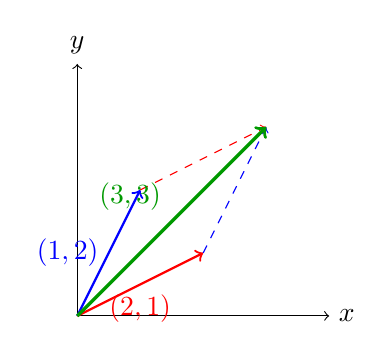
\begin{tikzpicture}[scale=0.8]
          \draw[->] (0,0) -- (4,0) node[right] {$x$};
          \draw[->] (0,0) -- (0,4) node[above] {$y$};
          \draw[->,blue,thick] (0,0) -- (1,2) node[midway,left] {$(1,2)$};
          \draw[->,red,thick] (0,0) -- (2,1) node[midway,below] {$(2,1)$};
          \draw[->,blue,dashed] (2,1) -- (3,3);
          \draw[->,red,dashed] (1,2) -- (3,3);
          \draw[->,green!60!black,very thick] (0,0) -- (3,3) node[midway,above left] {$(3,3)$};
        \end{tikzpicture}
      \end{center}
    \end{column}
  \end{columns}
\end{frame}

\begin{frame}[fragile]\frametitle{Scalar Multiplication}
  \begin{itemize}
    \item Multiply vector by a number (scalar)
    \item Example: $5 \cdot (2,1) = (10,5)$
    \item \textbf{Stretching}: multiply by $\alpha > 1$
    \item Vector becomes longer in same direction
    \item \textbf{Squeezing}: multiply by $0 < \alpha < 1$
    \item Vector becomes shorter in same direction
    \item Negative $\alpha$: reverses direction
    \item Scaling operation preserves direction (except sign)
  \end{itemize}
\end{frame}

\begin{frame}[fragile]\frametitle{Vector Space Axioms}
  \begin{itemize}
    \item \textbf{Commutativity}: $\mathbf{u} + \mathbf{v} = \mathbf{v} + \mathbf{u}$
    \item \textbf{Zero vector}: $0 \cdot \mathbf{v} = \mathbf{0}$
    \item Note: left zero is scalar, right is zero vector
    \item \textbf{Identity}: $1 \cdot \mathbf{v} = \mathbf{v}$
    \item \textbf{Distributivity 1}: $\alpha(\mathbf{u} + \mathbf{v}) = \alpha\mathbf{u} + \alpha\mathbf{v}$
    \item \textbf{Distributivity 2}: $(\alpha + \beta)\mathbf{v} = \alpha\mathbf{v} + \beta\mathbf{v}$
    \item \textbf{Associativity}: $(\alpha\beta)\mathbf{v} = \alpha(\beta\mathbf{v})$
    \item These are fundamental properties, always satisfied
  \end{itemize}
\end{frame}

\begin{frame}[fragile]\frametitle{Examples: $\mathbb{R}^n$ Spaces}
  \begin{itemize}
    \item $\mathbb{R}^2 = \{(x,y) : x,y \in \mathbb{R}\}$
    \item Two-dimensional vectors, plane
    \item $\mathbb{R}^3 = \{(x,y,z) : x,y,z \in \mathbb{R}\}$
    \item Three-dimensional vectors, space
    \item $\mathbb{R}^7 = \{(x_1, x_2, \ldots, x_7) : x_i \in \mathbb{R}\}$
    \item Seven-dimensional vectors
    \item All are vector spaces over $\mathbb{R}$
    \item Addition and scalar multiplication defined component-wise
  \end{itemize}
\end{frame}

\begin{frame}[fragile]\frametitle{Examples: Polynomial Spaces}
  \begin{itemize}
    \item $\mathbb{R}[x]$: all polynomials in variable $x$
    \item Example: $3x^2 + 2x + 1$, $x^5 - 7x + 2$
    \item Degree can be arbitrarily large
    \item Infinite-dimensional vector space
    \item $\mathbb{R}[x,y]$: polynomials in two variables
    \item Example: $x^2y + 3xy^3 + 7$
    \item Addition: $(p + q)(x) = p(x) + q(x)$
    \item Scalar multiplication: $(\alpha p)(x) = \alpha \cdot p(x)$
    \item Coefficients are the "coordinates"
  \end{itemize}
\end{frame}

\begin{frame}[fragile]\frametitle{Examples: Function Spaces}
  \begin{itemize}
    \item Differential equations have function solutions
    \item Example: $\frac{dy}{dx} + y = 0$ has solution $y = Ce^{-x}$
    \item Collect all solutions: $\{Ce^{-x} : C \in \mathbb{R}\}$
    \item This forms a vector space
    \item Addition: $(f + g)(x) = f(x) + g(x)$
    \item Scalar multiplication: $(\alpha f)(x) = \alpha \cdot f(x)$
    \item Calculus studies function spaces
    \item Real analysis: abstract treatment of calculus
  \end{itemize}
\end{frame>

\begin{frame}[fragile]\frametitle{Summary}
  \begin{itemize}
    \item Abstract approach removes coordinate dependence
    \item Vector spaces: sets with addition and scalar multiplication
    \item Works for any dimension: finite or infinite
    \item Linear transformations preserve vector space structure
    \item Examples: $\mathbb{R}^n$, polynomials, functions
    \item Foundation for quantum mechanics
    \item Next: Dirac notation (bra-ket) for QM
    \item Everything learned here applies to quantum states
  \end{itemize}
\end{frame}
